\section{De projectorganisatie}
Iedere dinsdag, tot aan het afronden van het project, houden we bijeenkomsten om alle zaken te bespreken en gezamenlijk te werken. Bovendien zullen we doordeweeks op afstand aan het project blijven werken.

Voor het opstellen van onze projectdocumentatie maken we gebruik van LaTeX in de Overleaf-omgeving. Dit biedt ons veel flexibiliteit in het opmaakformaat van onze documenten.

Daarnaast hebben we een gedetailleerde planning waarin we een logboek bijhouden via onze Github. Meer informatie hierover is te vinden in hoofdstuk \ref{planning}.

Om een duidelijk overzicht te verkrijgen van de functies en de betrokken personen/bedrijven, hebben we een mindmap samengesteld:
\vspace{1cm} 
\begin{minipage}[t][][b]{\linewidth}
  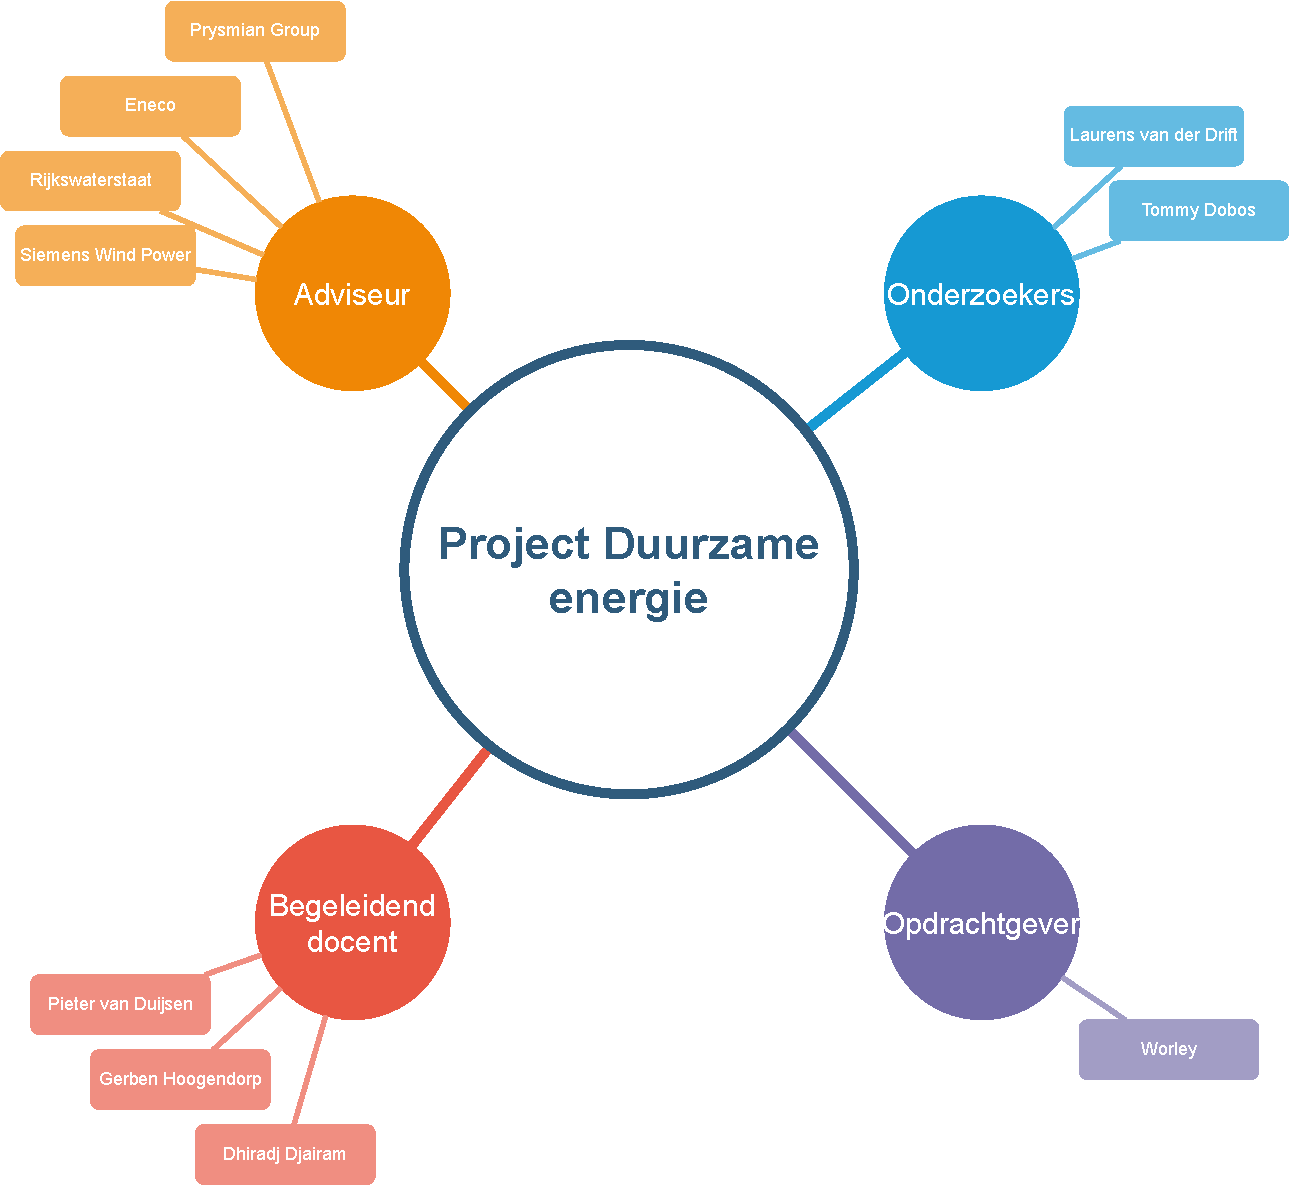
\includepdf[scale=0.65, pages=-]{mindmap/projectorganisatie.pdf}
\end{minipage}
% % Please add the following required packages to your document preamble:
% % \usepackage[table,xcdraw]{xcolor}
% % If you use beamer only pass "xcolor=table" option, i.e. \documentclass[xcolor=table]{beamer}
% \begin{table}[h]
% \begin{tabular}{|l|l|l|}
% \hline
% \rowcolor[HTML]{9B9B9B} 
% {\color[HTML]{FFFFFF} \textbf{Projectlid}} & {\color[HTML]{FFFFFF} \textbf{Functie}} & {\color[HTML]{FFFFFF} \textbf{Taak}} \\ \hline
% \rowcolor[HTML]{EFEFEF} 
% Laurens van der Drift & Leider & SonarSensor \\ \hline
%  &  & IR Sensor \\ \hline
%  &  & \cellcolor[HTML]{EFEFEF}PCB hat \\ \hline
%  &  & Motoren \\ \hline
% \rowcolor[HTML]{EFEFEF} 
% Francisco Ramirez Ramirez & Ontwerper & 3D   Ontwerp \\ \hline
%  &  & Servo's \\ \hline
%  &  & \cellcolor[HTML]{EFEFEF}Motoren \\ \hline
%  &  & Notuleren \\ \hline
% \rowcolor[HTML]{EFEFEF} 
% Justin   van der Reijden & Programmeur & SonarSensor \\ \hline
%  &  & IR Sensor \\ \hline
%  &  & \cellcolor[HTML]{EFEFEF}Notuleren \\ \hline
%  &  & Plannen \\ \hline
% \rowcolor[HTML]{EFEFEF} 
% Tommy Dobos & Documentaires & Motoren \\ \hline
%  &  & Servo's \\ \hline
%  &  & \cellcolor[HTML]{EFEFEF}Documenteren \\ \hline
%  &  & Eindredactie \\ \hline
% \end{tabular}
% \end{table}

% Na de taakverdeling volgt een planning. De projectgroep heeft gezamenlijk besloten om een standaard dag in te plannen waarop er een bijeenkomst plaatsvindt om het traject betreffende het project te bespreken. Deze afgesproken dag is elke donderdag van 9:30 tot 19:30 bijeenkomen om eventuele knelpunten en bijzonderheden met betrekking tot het bouwen van de zelf rijdende auto te bespreken. De bijeenkomsten zullen worden gehouden in een beschikbare ruimte van de Haagse Hoge School.  Indien alle ruimtes bezet zijn zal  het studielandschap gebruikt worden om daar verder te werken.

% Aan het einde van elke dag, een uur voor het opruimen, is er tijd ingepland om alles te noteren en documenteren wat gedurende die dag gedaan is aan het project. Dit zal gebeuren door middel van het programma Github.  